
\section{引言}
关于Chromium的多进程模型,无论是其官方文档,还是技术论坛都有许多说明。
所以,本文在此就不对多进程模型的框架再做过多的讲解。如果想了解这方面知识,请查阅官方文档中的多进程架构一节。
本文的重点在于研究Chromium各进程的启动流程、以及Render进程的启动策略。重点在于具体实现和具体流程的分析。

目前Chromium包含四类进程:Browser进程、Render进程、GPU进程和Plugein进程。
本文目前主要讨论Browser进程和Render进程,其他两类进程将在后续研究中添加。
Chromium也包含多个平台的实现,目前本文主要研究Windows平台和Linux平台,其他平台暂时不做研究。
Chromium可以编译为多个形式的应用,本文主要以比较简单的content\_shell作为研究对象。

\section{Chromium多进程模型简介}

\begin{figure}[H] 
  \centering 
  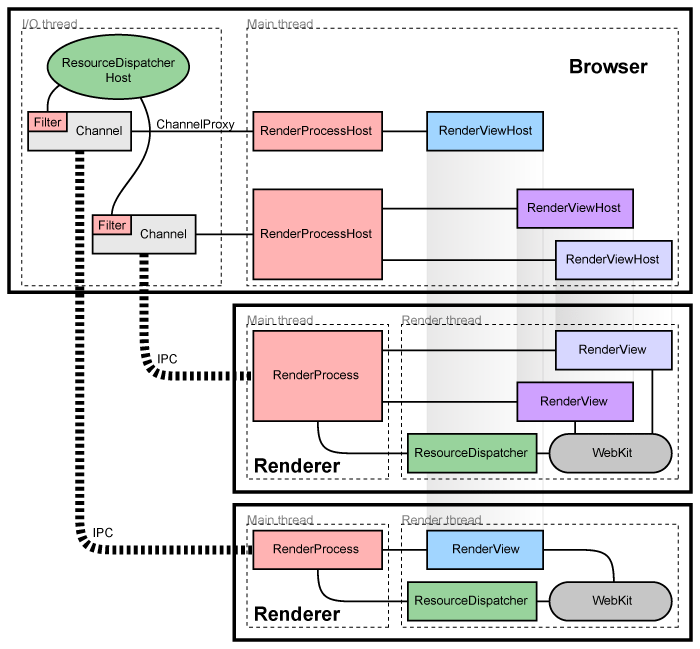
\includegraphics[width=0.80\textwidth]{image/process_study/multi_process_architecture.png} 
  \caption{chromium多进程模型示意图} \label{fig:multi_process_architecture} 
\end{figure}

如图~\ref{fig:multi_process_architecture}所示,是chromium官方文档给出的多进程模型的简单示意图。
图中主要描绘了Browser进程和Render进程的关系。
其中,最上面的那个方框代表Browser主进程,是UI所在的进程,负责与用户交互、处理网络请求和管理Render进程等。
从图中可以看出,Render进程可以不止一个,它主要任务是渲染打开的网页。
但是并不能简单的理解为一个网页就是一个Rander进程,这个关系是可以通过启动参数配置的,后面会详细讨论这个问题。

可以从图中看出,Browser进程是通过RenderProcessHost和RenderProcess对象管理Render进程的。
RenderProcessHost对象与Render进程中的RenderProcess对象一一对应。
每一个Render进程都有且只有一个全局的RenderProcess对象,Render进程可以通过它和Browser进程通信。

每个Render进程都会有一个或多个RenderView对象,它们受RenderProcess对象管理,代表一个使用WebKit引擎渲染的区域。
同样,在Browser进程中的RenderProcessHost对象管理着与RenderView对应的RenderViewHost对象。
在chromium中,还存在RenderWidgetHost和RenderWidget类,作为RenderViewHost和RenderView父类。
RenderProcess、RenderWidge、RenderView对Browser和Render进程之间的消息传递具有重要的作用,后续的章节会作出详细的研究。

在Chromium启动之初,最先启动的是Browser进程,由它来启动其他进程。
这四类进程中Browser进程和GPU进程都只会有一个,而Render进程和插件进程可以存在多个。
另外,Chromium提供了启动参数可以设置为单进程模式,就是所有的功能运行在一个进程中。

\section{Browser进程启动流程}
Browser作为Chromium系统的主进程,最先启动。
其启动的流程自然从main函数开始的。
Browser进程的main函数非常简单,它定义在shell\_main.cc中,其代码如下:

\begin{spacing}{1.0}
\begin{lstlisting}[language={C++}]
int main(int argc, const char** argv) {
#if defined(OS_MACOSX)
  // Do the delegate work in shell_content_main to avoid having to export the
  // delegate types.
  return ::ContentMain(argc, argv);
#else
  content::ShellMainDelegate delegate;
  content::ContentMainParams params(&delegate);
  params.argc = argc;
  params.argv = argv;
  return content::ContentMain(params);
#endif  // OS_MACOSX
}
\end{lstlisting}
\end{spacing}

在这段代码中定义了两个对象,它们的类型是ShellMainDelegate与ContentMainParams,最后调用了ContentMain函数。
ContentMain函数也是非常简单的:

\begin{spacing}{1.0}
\begin{lstlisting}[language={C++}]
int ContentMain(const ContentMainParams& params) {
  std::unique_ptr<ContentMainRunner> main_runner(ContentMainRunner::Create());

  int exit_code = main_runner->Initialize(params);
  if (exit_code >= 0)
    return exit_code;

  exit_code = main_runner->Run();

  main_runner->Shutdown();

  return exit_code;
}
\end{lstlisting}
\end{spacing}

从以上的代码可以看出,Browser进程启动之初,最终是执行了ContentMainRunner接口的Run方法。
其实,不止Browser进程,其他进程也同样会执行这段代码,那么就让我们分析一下这些类以及后续的调用流程吧。

\begin{figure}[H] 
  \centering 
  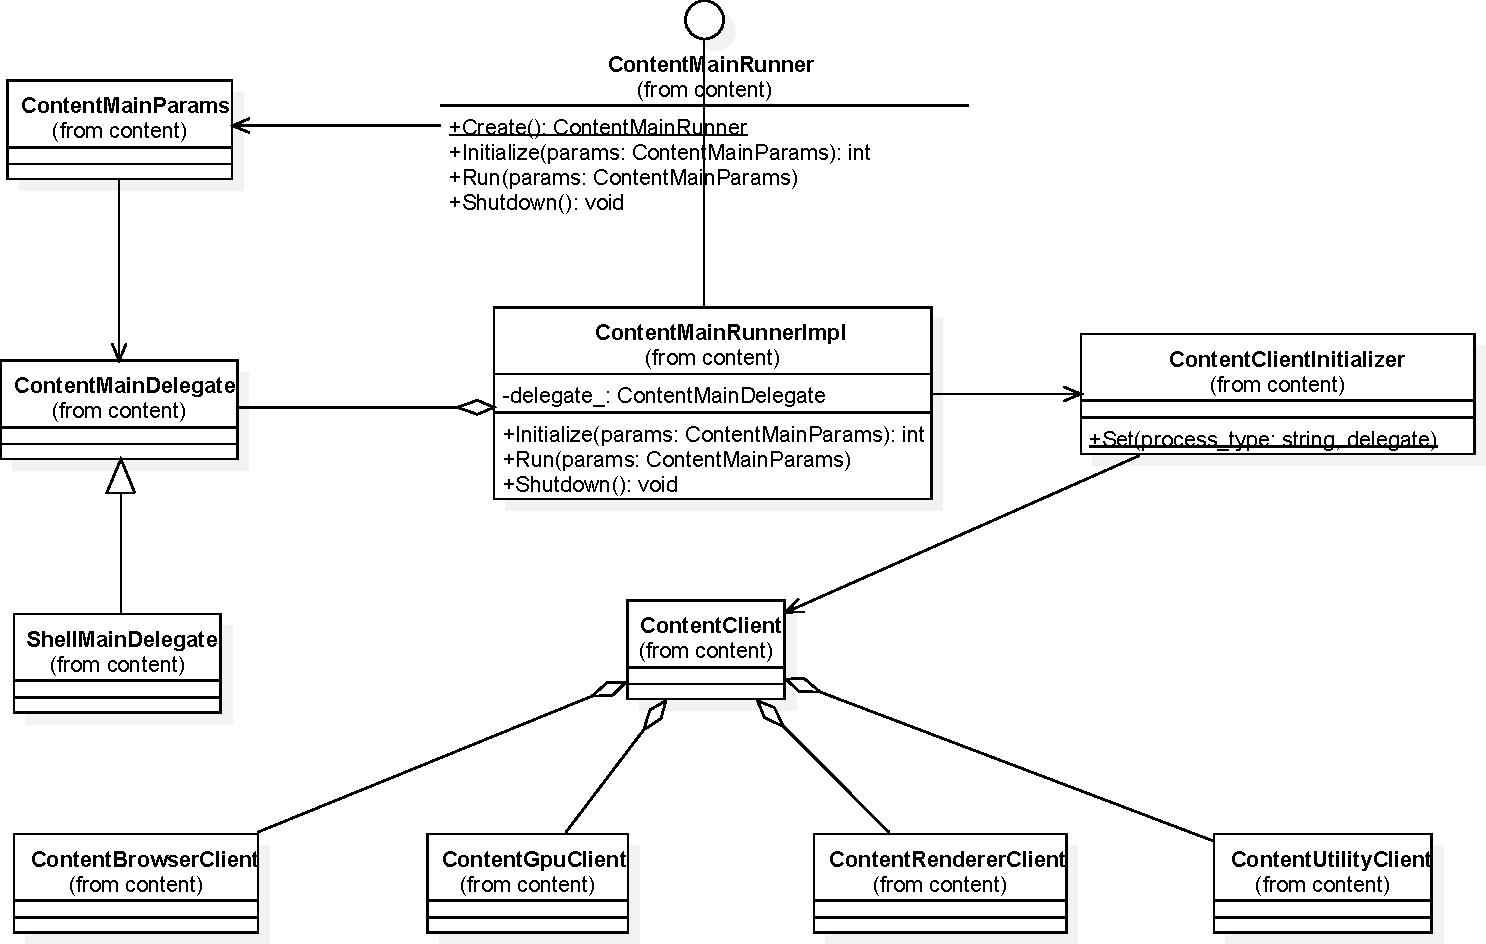
\includegraphics[width=0.90\textwidth]{image/process_study/ContentMainRunner.pdf} 
  \caption{ContentMainRunner相关类图} \label{fig:ContentMainRunnerClass} 
\end{figure}

如图~\ref{fig:ContentMainRunnerClass}所示,ContentMainRunnerImpl是ContentMainRunner接口的实现类,
也是这个过程中主要的工作对象,其生命周期与Browser进程的生命周期相同。
在创建过程中,将用到ContentMainParams对象和ShellMainDelegate对象。

在ContentMainRunnerImpl的Initialize函数中,还会调用ContentClientInitializer的Set函数,
向一个全局的ContentClient对象中设置一个ContentBrowserClient对象。
这个对象有许多的功能,在Browser进程的多个节点都可以作出一些影响。
如:当要打开某个URL时,决定是否真的要打开;遇到证书错误时,作出相应的策略选择;是否允许某个网站使用AppCache功能等。

\begin{figure}[H] 
  \centering 
  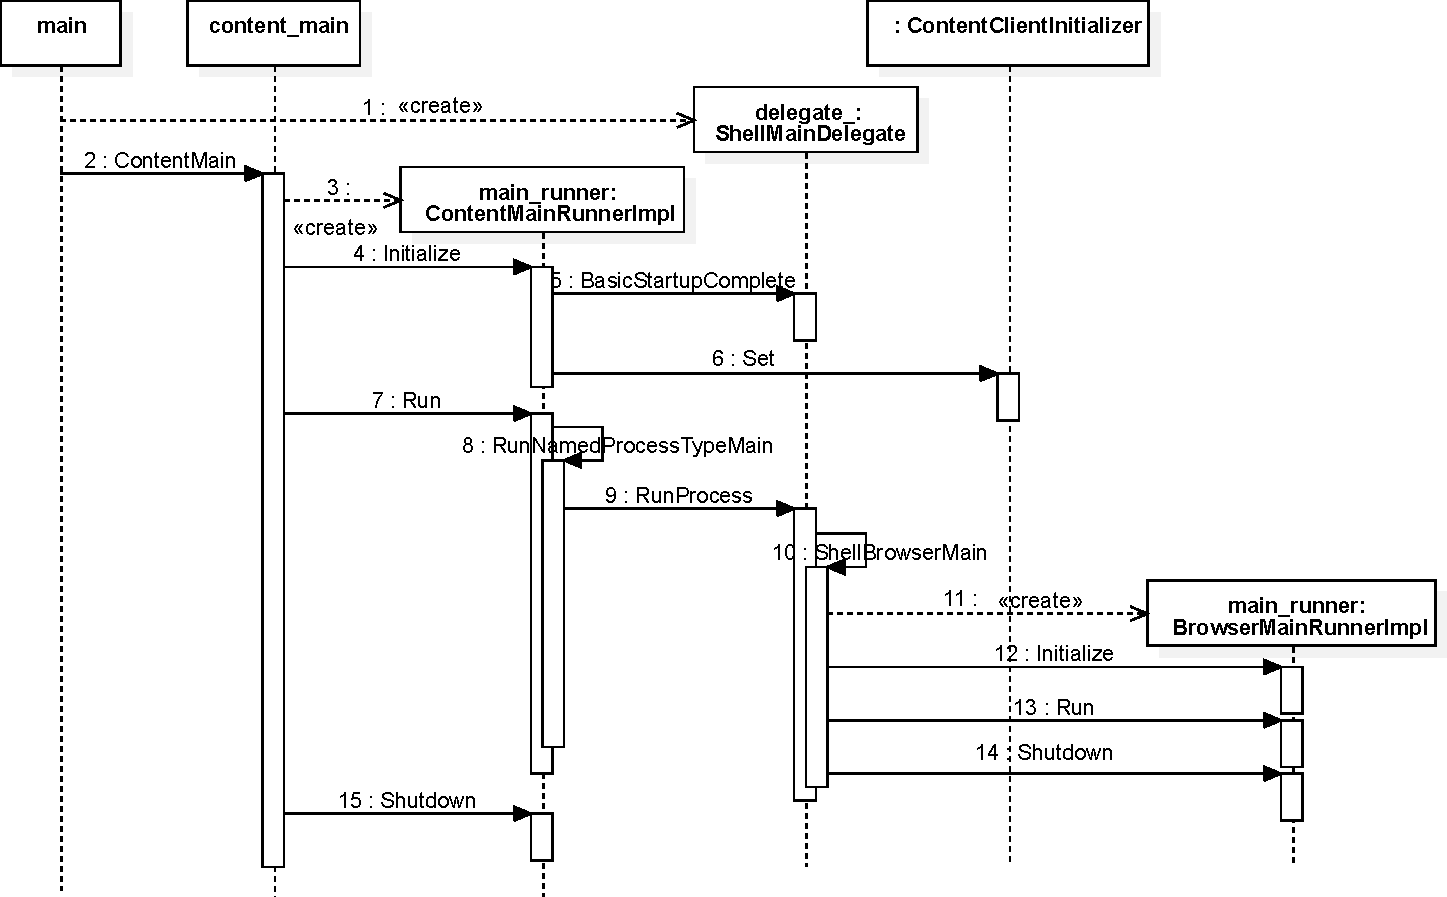
\includegraphics[width=0.90\textwidth]{image/process_study/ContentMainRunnerSequence.pdf} 
  \caption{浏览器进程启动初始流程} \label{fig:ContentMainRunnerSequence} 
\end{figure}

如图~\ref{fig:ContentMainRunnerSequence},是浏览器进程从开始启动,到真正按进程类型去执行相关的功能的时序图。其中:
\begin{itemize}
  \item 在ContentMainRunnerImpl类的Initialize方法中做进程启动的准备工作。
  如:调用delegate\_对象的BasicStartupComplete,在此方法中初始化log模块;
  调用ContentClientInitializer类的Set方法,设置进程的ContentClient,等等。
  \item 随着Run方法的调用,进程开始运转。Run方法的执行一直持续到整个进程结束。
  方法后续调用了RunNamedProcessTypeMain函数,进入根据不同进程类型执行不同代码的逻辑。
  也就是说,在此之前,所有的进程的逻辑都是相同的,这一点在后续的章节将要描述。
\end{itemize}





BrowserMainRunner
BrowserMainRunnerImpl

BrowserMainLoop
ShellBrowserMainParts


ContentClient
ShellContentBrowserClient
ContentRendererClient
可以对浏览器的诸多流程做出控制,与confige关联密切

浏览器Browser进程启动后,直接运行UI线程,UI线程又创建其他6个线程
在BrowserMainLoop::CreateThreads函数中创建浏览器其他线程


\section{Render进程启动流程}

为什么设置的log在render进程中失效

\section{Render进程的启动策略}

\section{Browser进程和Render进程重要类的对应关系}
